\documentclass[border=8pt]{standalone}
\usepackage[T1]{fontenc}\usepackage[utf8]{inputenc}
\usepackage{helvet}\renewcommand{\familydefault}{\sfdefault}
\usepackage{tikz,xcolor}
\usetikzlibrary{arrows.meta,positioning,shapes.geometric,shapes.multipart,calc,fit,backgrounds,decorations.markings}
\definecolor{ink}{HTML}{1E1B16}\definecolor{paper}{HTML}{FBF8F2}\definecolor{clay}{HTML}{B5482A}\definecolor{soft}{HTML}{F1E9DA}\definecolor{pine}{HTML}{24402F}
\tikzset{
  every node/.style={font=\small,text=ink},
  >=Stealth, line/.style={draw=ink,line width=0.8pt},
  cls/.style={rectangle split,rectangle split parts=3,draw=ink,line width=0.8pt,fill=soft,align=left,inner xsep=6pt,inner ysep=4pt,
              rectangle split part align={center,left,left},minimum width=3.0cm},
  cls2/.style={rectangle split,rectangle split parts=2,draw=ink,line width=0.8pt,fill=soft,align=left,inner xsep=6pt,inner ysep=4pt,
              rectangle split part align={center,left},minimum width=3.0cm},
  box/.style={rectangle,draw=ink,line width=0.8pt,fill=soft,align=center,inner sep=5pt,minimum height=0.8cm},
  state/.style={rectangle,rounded corners=8pt,draw=ink,line width=0.8pt,fill=soft,align=center,inner sep=6pt,minimum width=2.2cm,minimum height=0.9cm},
  act/.style={rectangle,rounded corners=10pt,draw=ink,line width=0.8pt,fill=soft,align=center,inner sep=5pt,minimum width=2.4cm,minimum height=0.8cm},
  dec/.style={diamond,draw=ink,line width=0.8pt,fill=soft,inner sep=1pt,minimum width=0.9cm,minimum height=0.9cm},
  uc/.style={ellipse,draw=ink,line width=0.8pt,fill=soft,align=center,inner sep=3pt,minimum width=3.2cm,minimum height=1.0cm},
  note/.style={rectangle,draw=ink,line width=0.6pt,fill=yellow!12,align=left,inner sep=4pt,font=\footnotesize},
  lab/.style={font=\footnotesize,fill=paper,inner sep=1.5pt},
  err/.style={},
}
\newcommand{\actor}[3]{% x,y,label
  \draw[line width=0.8pt] (#1,#2+0.55) circle (0.17);
  \draw[line width=0.8pt] (#1,#2+0.38)--(#1,#2-0.15) (#1-0.3,#2+0.22)--(#1+0.3,#2+0.22) (#1,#2-0.15)--(#1-0.25,#2-0.6) (#1,#2-0.15)--(#1+0.25,#2-0.6);
  \node[font=\small] at (#1,#2-0.9) {#3};}
\begin{document}
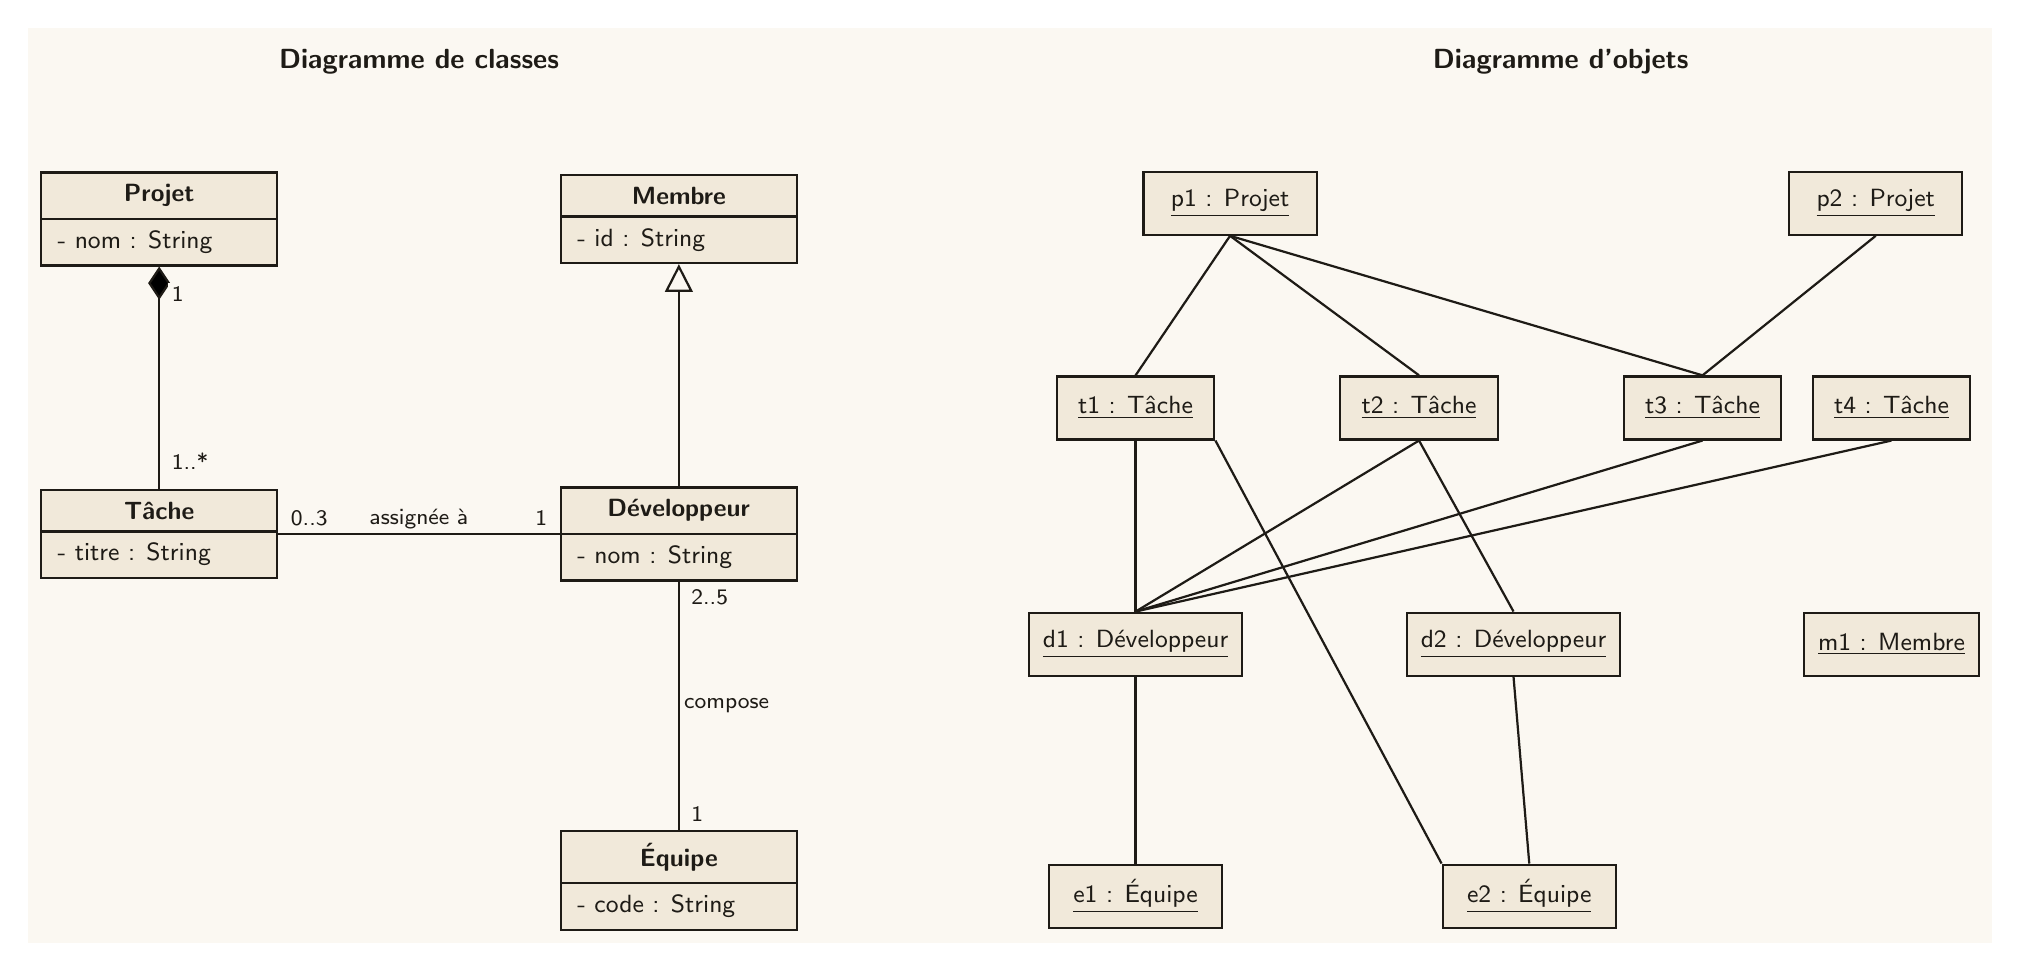
\begin{tikzpicture}[background rectangle/.style={fill=paper},show background rectangle]
\node[font=\bfseries] at (3.9,7.6) {Diagramme de classes};
\node[cls2,minimum width=3.0cm] (P) at (0.6,5.6) {\textbf{Projet}\nodepart{two}- nom : String};
\node[cls2,minimum width=3.0cm] (T) at (0.6,1.6) {\textbf{Tâche}\nodepart{two}- titre : String};
\node[cls2,minimum width=3.0cm] (D) at (7.2,1.6) {\textbf{Développeur}\nodepart{two}- nom : String};
\node[cls2,minimum width=3.0cm] (E) at (7.2,-2.8) {\textbf{Équipe}\nodepart{two}- code : String};
\node[cls2,minimum width=3.0cm] (M) at (7.2,5.6) {\textbf{\textit{Membre}}\nodepart{two}- id : String};
\draw[line,{Diamond[length=12pt,width=8pt]}-] (P.south)--(T.north);
\node[lab,anchor=west] at ([xshift=0.1cm,yshift=-0.35cm]P.south) {1};
\node[lab,anchor=west] at ([xshift=0.1cm,yshift=0.35cm]T.north) {1..*};
\draw[line,] (T.east)--(D.west) node[midway,above,lab]{assignée à};
\node[lab,anchor=south west] at ([xshift=0.1cm,yshift=0.05cm]T.east) {0..3};
\node[lab,anchor=south east] at ([xshift=-0.1cm,yshift=0.05cm]D.west) {1};
\draw[line,] (D.south)--(E.north) node[midway,right,lab]{compose};
\node[lab,anchor=north west] at ([xshift=0.1cm,yshift=-0.05cm]D.south) {2..5};
\node[lab,anchor=south west] at ([xshift=0.1cm,yshift=0.05cm]E.north) {1};
\draw[line,-{Triangle[open,length=10pt,width=10pt]}] (D.north)--(M.south);
\node[font=\bfseries] at (18.4,7.6) {Diagramme d'objets};
\node[box,minimum width=2.2cm] (p1) at (14.2,5.8) {\underline{p1 : Projet}};
\node[box,minimum width=2.2cm] (p2) at (22.4,5.8) {\underline{p2 : Projet}};
\node[box,minimum width=2.0cm] (t1) at (13.0,3.2) {\underline{t1 : Tâche}};
\node[box,minimum width=2.0cm] (t2) at (16.6,3.2) {\underline{t2 : Tâche}};
\node[box,minimum width=2.0cm] (t3) at (20.2,3.2) {\underline{t3 : Tâche}};
\node[box,minimum width=2.7cm] (d1) at (13.0,0.2) {\underline{d1 : Développeur}};
\node[box,minimum width=2.7cm] (d2) at (17.8,0.2) {\underline{d2 : Développeur}};
\node[box,minimum width=2.2cm] (m1) at (22.6,0.2) {\underline{m1 : Membre}};
\node[box,minimum width=2.2cm] (e1) at (13.0,-3.0) {\underline{e1 : Équipe}};
\node[box,minimum width=2.2cm] (e2) at (18.0,-3.0) {\underline{e2 : Équipe}};
\node[box,minimum width=2.0cm] (t4) at (22.6,3.2) {\underline{t4 : Tâche}};
\draw[line] (p1.south)--(t1.north);
\draw[line] (p1.south)--(t2.north);
\draw[line] (p1.south)--(t3.north);
\draw[line] (p2.south)--(t3.north);
\draw[line] (t1.south)--(d1.north);
\draw[line] (t2.south)--(d1.north);
\draw[line] (t2.south)--(d2.north);
\draw[line] (t4.south)--(d1.north);
\draw[line] (t3.south)--(d1.north);
\draw[line] (d1.south)--(e1.north);
\draw[line] (d2.south)--(e2.north);
\draw[line] (t1.south east)--(e2.north west);
\end{tikzpicture}
\end{document}
